\chapter{Grundlagen}
\label{ch:Grundlagen}
Im Gegensatz zu weiten Teilen der Informatik besteht in der Telekommunikation seit langem die Notwendigkeit, herstellerunabhangige und präzise Standards für Kommu- nikationsprotokolle und -dienste zu erstellen. Diese Anforderung hat dazu gefuhrt, dass man sich schon frühzeitig mit der Entwicklung der formalen Modellierungssprachen Message Sequence Chart (MSC) und Specification and Description Language (SDL) beschaftigt hat. Im Gegensatz etwa zur Unified Modeling Language (UML) liegt MSC und SDL eine formale Semantik zugrunde, die die Bedeutung der einzelnen Sprachkonstrukte klar und eindeutig mathematisch definiert.\\
MSC und SDL sind von der International Telecommunication Union standardisiert worden. Fur beide Sprachen existieren eine graphische Reprasentation (MSC /GR bzw. SDL/GR) fur die Benutzung durch Menschen und eine textuelle Notation (MSC/PR bzw. SDL/PR) fur eine maschinelle Weiterbearbeitung. MSC und SDL werden haufig gemeinsam im Software-Entwicklungsprozess eingesetzt. MSC dient dabei zur Anforderungsdefinition, Testfallspezifikation und Dokumentation, wahrend SDL in der Spezifikationsphase und der Implementierungsphase eingesetzt wird.

\section{\acf{SDL}}
\label{sc:SDL}
Die \acs{SDL} (\ac{SDL}, engl. Spezifikations und Beschreibungssprache) ist eine von der \ac{ITU-T} (\ac{ITU-T}, engl. Internationalen 
Telekommunikations- Vereinigung für Standardisierung der Telekommunikation) standardisierte objektorientierte Modellierungssprache. Die erste Version wurde erstmalig 
1976 definiert und die aktuellste Version von \ac{SDL} ist \ac{SDL}-2010 aus dem Jahre 2007, welche eine Überarbeitung der \ac{SDL}-Version \ac{SDL}-2000 aus dem Jahre 
1999 ist \cite[vii,51]{ITUT100_2016}. Wenn im folgenden von \ac{SDL} gesprochen wird, wird immer die Version \acs{SDL}-2010 gemeint. 
\ac{SDL} wird zur Beschreibung von Telekommunikationssystemen, deren Abläufe, sowie für Protokoll Definitionen und in verteilten Systemen eingesetzt.
Der Anwendungsbereich erstreckt sich über komplexe ereignisgesteuerte, interaktiven Echtzeitanwendungen, welche über Nachrichten miteinander kommunizieren. 
Der Hauptfokus von \ac{SDL} ist, sich einen genauen Überblick über das Verhalten genannter Systeme zu machen, wobei Eigenschaften mit anderen Techniken beschrieben werden müssen \cite[1\psq]{ITUT100_2016}. 
So wird \ac{MSC} unter anderem zum Beschreiben von Interaktionsverhalten zwischen Systemen, \ac{ASN1} für die Beschreibung von Datentypen und \ac{TTCN3} für Tests verwendet. In den letzten Überarbeitungen wurde die Spezifikation von \ac{SDL} um objekt-orientierte Aspekte erweitert und mit Sprachen wie \ac{UML} und \ac{ASN1} harmonisiert \cite[vii\psqq]{ITUT100_2016}. \ac{SDL} kann entweder grafisch oder textuell beschrieben werden. Beide Notationen sind semantisch äquivalent und lassen sich ineinander überführen \cite[3]{Weber_2008}. Folgende Abbildung veranschaulicht dies beispielhaft:

\begin{figure}[h]
	\centering
	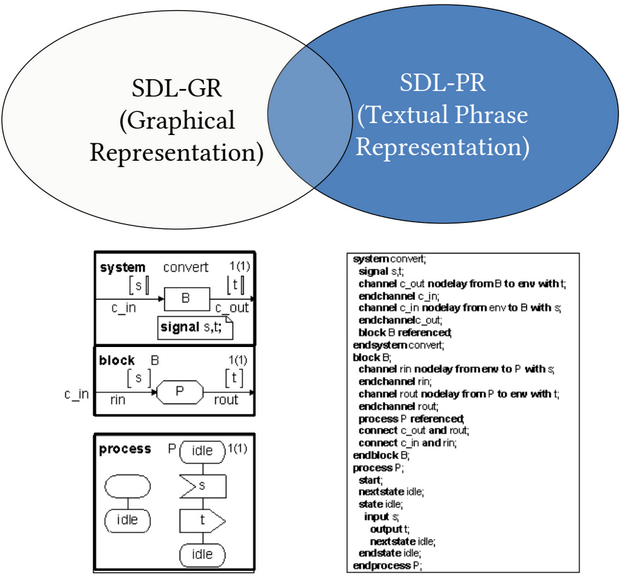
\includegraphics[width=0.5\textwidth]{Graphics/TextUndGrafik.png}
	\caption{Textuelle und Grafische Repräsentation : Quelle \cite{Reed_2000}}
	\label{fig:TextUndGrafik}
\end{figure}

\subsection{Architektur}
\label{ssc:Architektur}
Die \ac{SDL}-Spezifikation beschreibt ein hierarchisches System und erlaubt die strukturierte Trennung in Diagramme und Pakete und somit ein aufteilen eines Systems in viele kleinere Teilsysteme. Dies wirkt sich positiv auf die Entwicklung eines Systems in größeren Gruppen aus und vereinfacht diese. Ein System ist eine Menge an Blöcken, welche über Kanäle miteinander und der Umgebung außerhalb des Systems verbunden sind. Ein Kanal besitzt die Namen der Nachrichten bzw. Signale, welche über ihn übertragen werden können. Blöcke können Mengen von weiteren Blöcken enthalten oder als Prozess verfeinert dargestellt werden. Ebenso können Prozesse eine Menge von Prozessen in sich definiert haben.
Ein Prozess ist auf der untersten hierarchischen Ebene und beschreibt das dynamische Systemverhalten. Dies wird durch endliche Automaten, den \ac{EFSM} beschrieben. Diese besitzen abstrakte Datentypen und Merkmale von Objektorientierung \cite[3\psq]{ITUT100_2016}. Diese Strukturhierarchie wird anhand folgender Abbildung \ref{fig:Agenten} veranschaulicht.
 
\begin{figure}[h]
	\centering
	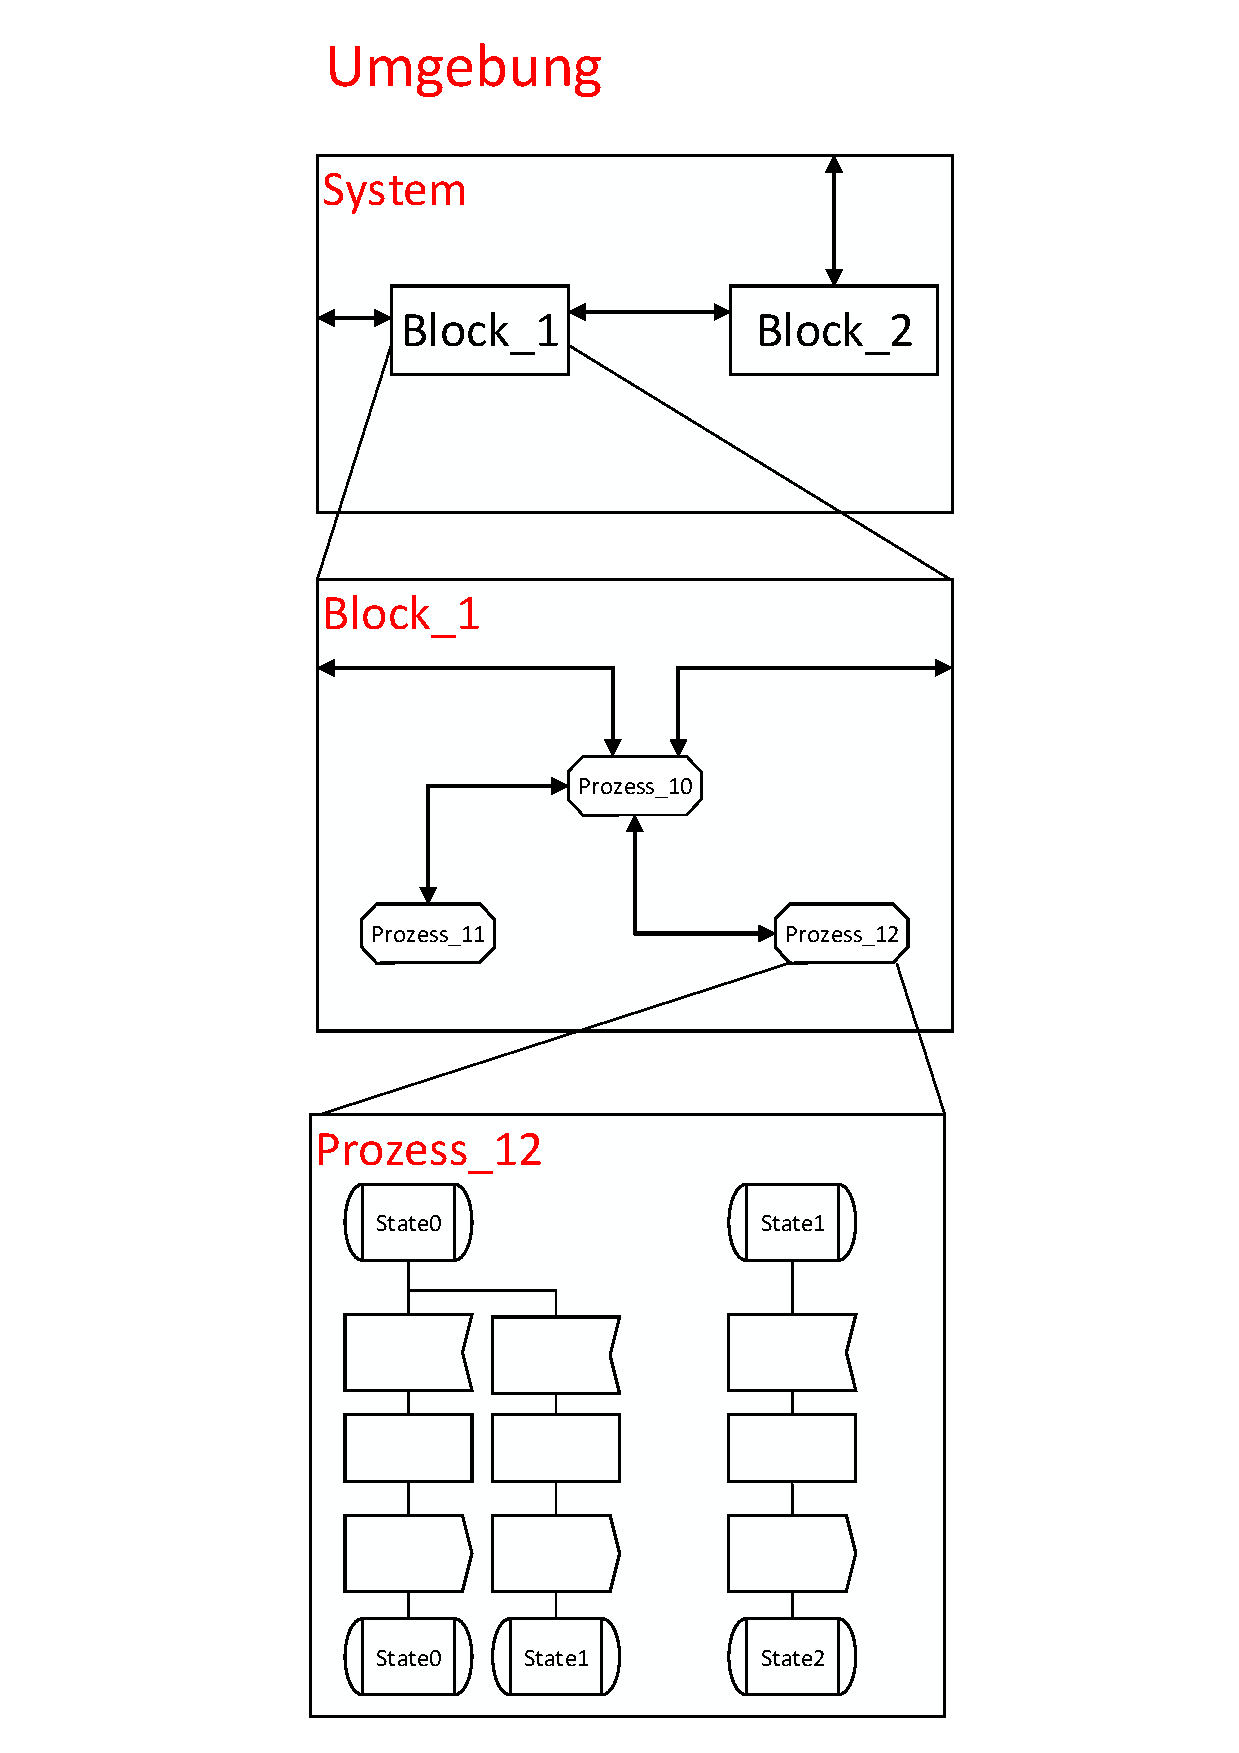
\includegraphics[width=0.6\textwidth]{Graphics/Agenten.pdf}
	\caption{SDL Architekturhierarchie}
	\label{fig:Agenten}
\end{figure}
\pagebreak
\subsubsection{Agenten}
Seit \ac{SDL}-2000 werden alle Funktionsblöcke übergreifend als Agenten bezeichnet. Der System-Agent, ist ein speziell ausgezeichneter Block-Agent. Er beinhaltet weitere Block-Agenten und definiert die Nachrichten mit denen über die Umgebung kommuniziert wird. Block- und Prozess-Agenten unterscheiden sich in über die Kontrolle ihrer Ausführungsart. Wo die Zustandsmaschinen von Block-Agenten nebenläufig ablaufen können, müssen Prozess-Agenten auf den Abschluss der in Ausführung befindlichen Transaktion warten um ihren Zustand wechseln zu können \cite[29\psq]{ITUT101_2016}.


\subsection{Kommunikation}
\label{ssc:Kommunikation}
Die Kommunikation innerhalb von \ac{SDL} findet asynchron über Nachrichten bzw. mit diskreten Signalen (in \ac{SDL} signals) über Kanäle (in \ac{SDL} channel) statt. 
Diese können sowohl auf Systemebene, als auch auf Blockebene definiert werden und verbinden die Agenten untereinander oder mit der Umgebung.
Jeder Kanal besitzt einen Namen, genauso wie Nachricht aber auch optionale Parameter besitzen und in eine Liste gruppiert werden können.
Ein Kanal besteht immer aus einer Quelle und einem Endpunkt. Kanäle werden entweder Bi- oder Unidirektional definiert. Dabei kann ein Kanal verzögert oder nicht verzögert wirken und demnach Nachrichten verzögert ankommen. Der Kanal muss entweder in einem anderen Agenten oder in die Umgebung (in \ac{SDL} environment) enden. Er kann aber auch den innerbefindlichen Prozess eines Agenten mit der Umgebung bzw. mit einem anderen innerbefindlichen Agenten verbinden \cite[39-42]{ITUT101_2016}. Dabei ist die Umgebung alles, was in einer \ac{SDL} spezifischen Sprache mit dem System kommunizieren kann \cite[3\psq]{ITUT100_2016}.
Abbildung \ref{fig:KommModell} zeigt die verschiedenen Kanäle beispielhaft:
 
\begin{figure}[h]
	\centering
	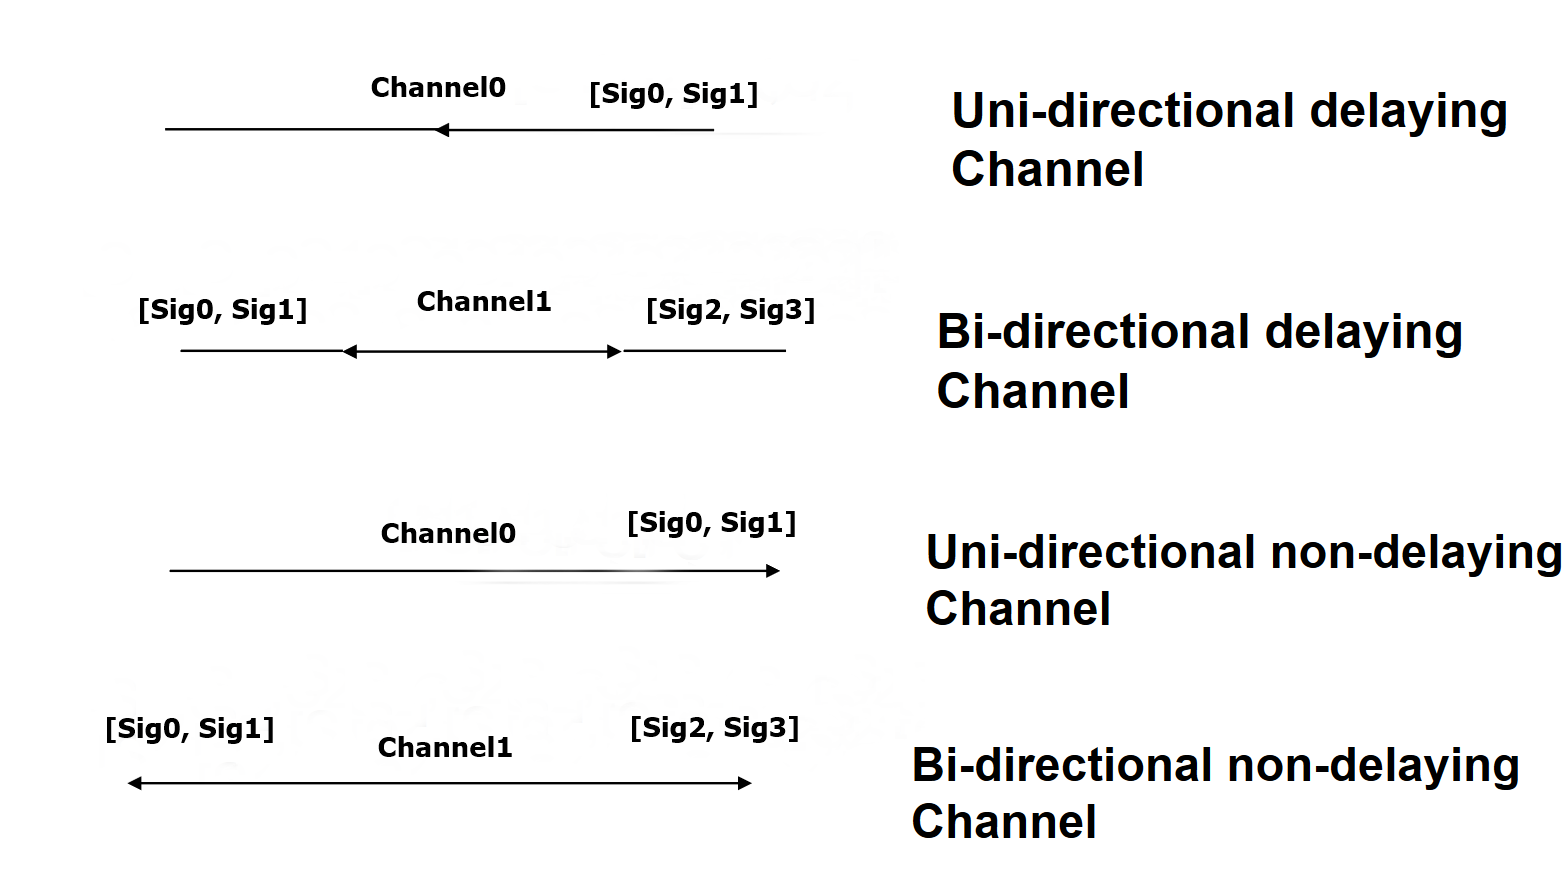
\includegraphics[width=0.6\textwidth]{Graphics/Channel.png}
	\caption{Verzögerte und nicht verzögerte Kanäle in SDL}
	\label{fig:KommModell}
\end{figure}

\subsection{Systemverhalten}
\label{ssc:Verhalten}
Das Verhalten von \ac{SDL} wird in Prozessen definiert, welche automatenbasiert und wie eben besprochen, mittels \ac{EFSM}s repräsentiert werden. Sie bestehen aus einer Menge an Zustandsübergängen, welche Beispielhaft in Abbildung \ref{fig:Basiskonstrukte} zu sehen sind. Darunter gehören Zustände wie Start, Bedingung, Eingabe und Ausgabe. Da eine Aufzählung dem Sinn der Arbeit nicht dienlich ist, wird in diesem Zusammenhang auf die Spezifikation verwiesen \cite[44 \psqq]{ITUT101_2016}.


Ein Prozess besitzt eine Prozess-Id (in \ac{SDL} PId), damit bei Instanziierung eines Prozesses, diese unterschieden werden können. Zusätzlich besitzt er einen Eingabepuffer zum Speichern von Nachrichten. Dieser Puffer übergibt nach dem \ac{FIFO}-Prinzip nacheinander die anstehenden Nachrichten des verbundenen Kanals an den Prozess \cite[42]{ITUT101_2016}. Abbildung \ref{fig:ProcessInit} zeigt einen Prozess beispielhaft. Kommen zwei Nachrichten von mehreren Kanälen gleichzeitig an einem Prozess an, so ist das Systemverhalten undefiniert und nach dem Zufall wird eine der beiden Nachrichten zuerst ausgeführt.
Die Modellierung der Automaten richtet sich oft nach Mealy, wobei in diesem die Ausgabe von seinem Zustand und seiner Eingabe abhängt.
Im Gegensatz zu Moore-Automaten enthält er keinen Startzustand, wobei jeder Mealy-Automat in einen Moore-Automat übertragen werden kann.
\begin{figure}[ht]
	\centering
	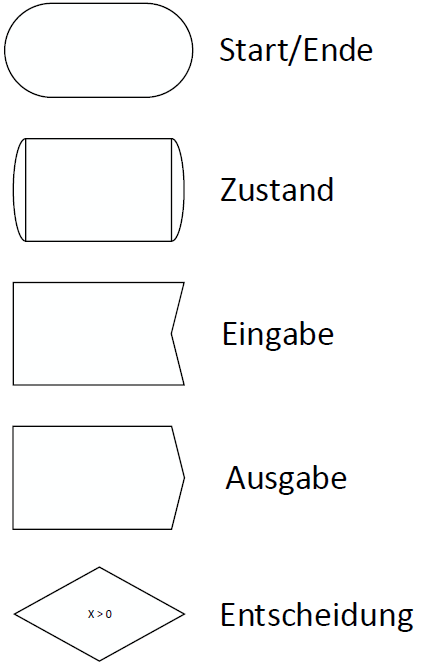
\includegraphics[width=0.3\textwidth]{Graphics/Basiskonstrukte.png}
	\caption{SDL-Basiskonstrukte}
	\label{fig:Basiskonstrukte}
\end{figure}

\begin{figure}[h]
	\centering
	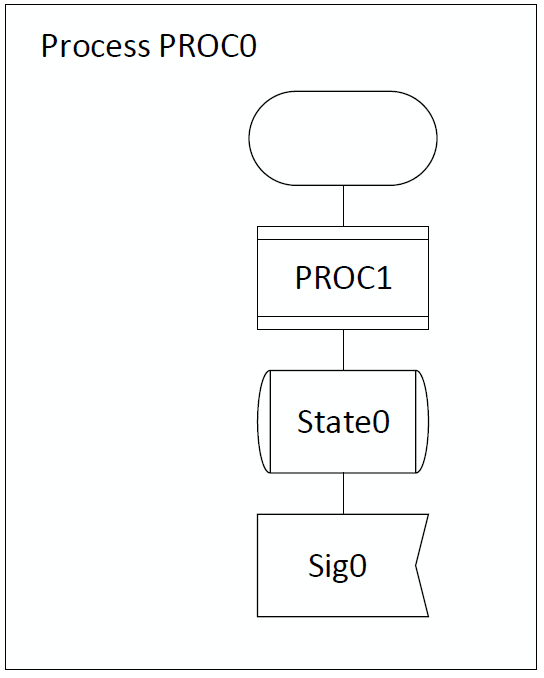
\includegraphics[width=0.5\textwidth]{Graphics/ProcessInit.png}
	\caption{SDL-Prozessinitialisierung}
	\label{fig:ProcessInit}
\end{figure}


\pagebreak
\subsection{Daten}
\label{ssc:Daten}
In \ac{SDL} können Daten auf zwei Arten beschrieben werden, einerseits mit dem \acs{ADT} oder mit \ac{ASN1}. \ac{ADT} definiert keine Datenstrukturen, sondern jeweils einen Satz (in \ac{SDL} sorts) an Werten, Operation und Bedingungen \cite[67]{ITUT104_2016}. In \ac{ADT} sind einige Datentypen wie Boolean, Character, Charstring, Integer und Real vordefiniert, aber auch Konstrukte wie Array und Enum. Eine Liste der vordefinierten Datentypen kann aus der Spezifikation entnommen werden \cite[47\psqq]{ITUT104_2016}. Neue Datentypen lassen sich durch bereits vorhandene Datentypen definieren, hierzu sind Einschränkungen und ein Standardwert in der Definition mit anzugeben. Abbildung \ref{fig:DatentypDef} verdeutlicht dies in einem Beispiel. In jedem Agenten lassen sich Konstanten, basierend auf den gewählten Datentypen definieren. Sie müssen einen konstanten Wert enthalten und dürfen nicht verändert werden. Variablen können nur in Prozessen definiert werden, enthalten denselben Aufbau wie Konstanten und können nur in ihrem definierten Prozess geändert werden. Zwar sind keine globalen Variablen zulässig, jedoch können Prozesse eigene Variablen anderen Prozessen sichtbar gemacht werden. Diese Variablen nennt man remote variables \cite[31]{ITUT102_2016}.

\begin{figure}[h]
	\centering
	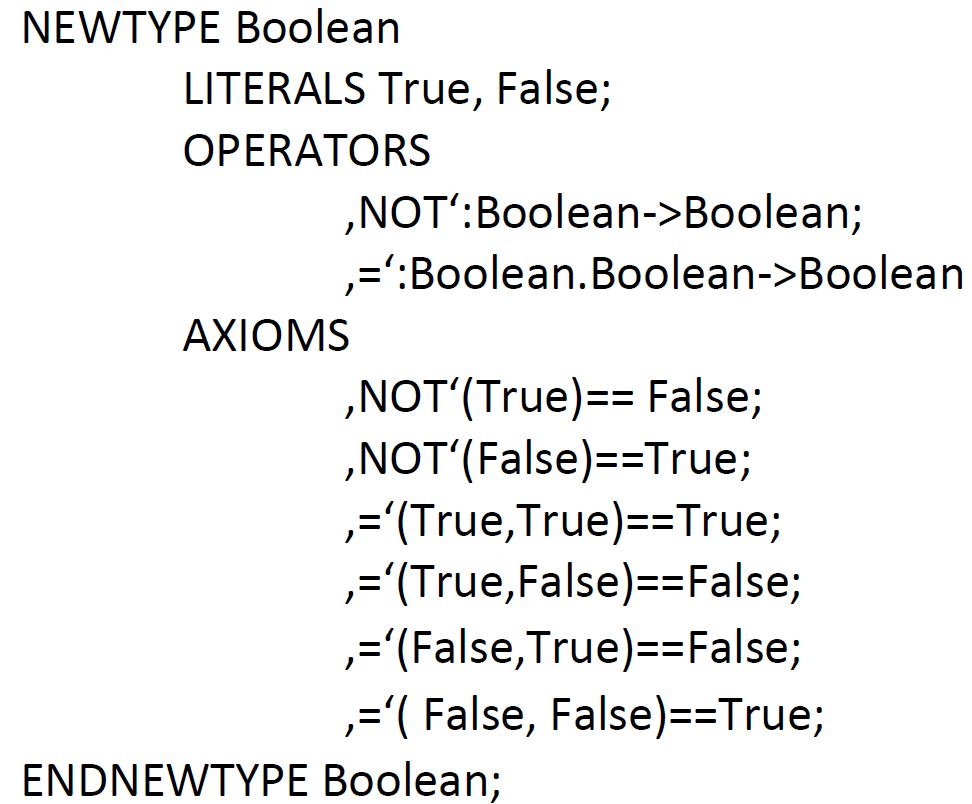
\includegraphics[width=0.5\textwidth]{Graphics/Data.png}
	\caption{SDL-Datentypdefinition}
	\label{fig:DatentypDef}
\end{figure}

Zu aller erst wird der Name des zu erstellenden Typs definiert. Dann das Set an Werten, welche verwendet werden dürfen. Und zu guter Letzt werden die Bedingungen des Typs definiert und mit dem Namen des erstellten Typs wieder abgeschlossen.

\pagebreak
\subsection{Objektorientierung} 
\label{ssc:Vererbung}
Die objektorientierten Konzepte von \ac{SDL} bieten dem Anwender eine Möglichkeit sein System zu strukturieren, wiederzuverwenden und das Modell ähnlicher der Realwelt abzubilden. So ist es möglich für einen Prozess-/Block-Agenten eine Prozess-/Block-Klasse zu erstellen. Im objektorientierten Ansatz werden diese auch als Typ (in \ac{SDL} type) bezeichnet. Diese werden für die Instanziierung, Vererbung und Spezialisierung von Typen verwendet. Ein Klassenagent kann auf jeder beliebigen Ebene definiert werden, egal ob nahe beim Kontext oder nicht.
Bei der Verwendung von Klassen, unterscheiden sich der objektorientierte und nicht-objektorientierte Ansatz syntaktisch zuerst nicht. Jedoch ist es möglich im objektorientierten Ansatz Instanzen der Klasse zu erzeugen \cite[4\psqq]{ITUT100_2016}.

\subsection{Spracheigenschaften}
\label{ssc:Spracheigenschaften}
Die Eigenschaften der Sprachdefinition von \ac{SDL} sind folgend beschrieben\cite[2\psq]{ITUT111_2016}:
\begin{itemize}{
		\item[Abstrakte Grammatik] Die abstrakte Grammatik von \ac{SDL} wird von einer abstrakten Syntax und statischen Bedingungen 
		beschrieben. Die Abstrakte Syntax kann entweder mit einer textbasierten Grammatik oder einem grafischen Metamodell erstellt werden.
		
		\item[Konkrete Grammatik] Die konkrete Grammatik wird durch eine grafische Syntax, statischen Bedingungen und Regeln für die grafische Syntax beschrieben.
		Beschrieben wird sie durch die erweiterte Backus-Naur Form. Wenn jedoch in der abstrakten Grammatik ein 
		grafisches Metamodell verwendet wurde, ist es erlaubt dieses um konkrete Eigenschaften zu erweitert und zu verwenden.
		
		\item[Semantik] Die Semantik gibt einem Konstrukt eine klare Bedeutung. Sie enthält dessen Eigenschaften, die Art der Interpretation und dynamischen Bedingungen die erfüllt sein müssen, damit das Konstrukt sich so verhält, sodass es in der Art verhält wie die Sprache gestaltet wurde. Die Eigenschaften sind wohl definierte Beziehungen, zwischen verschiedenen Konzepten.
		
		\item[Model] Das Model gibt Notationen eine Abbildungsform, wenn diese keine direkte abstrakten Syntax besitzen. Diese sind dann nach der konkreten Syntax anderer Konstrukte zu modellieren. Diese Konstrukte werden als \dq shorthand\dq bezeichnet und  beinhalten die Syntax der transformierten Form.
}\end{itemize}

\subsubsection{Metamodell}
\label{ssc:Metamodell}
Es werden derzeit Anstrengungen unternommen ein öffentlich zugängliches Metamodell von \ac{SDL} zu erstellen, welches alle Aspekte der Sprache in sich vereinigt. Zu dem derzeitigen Standpunkt existiert jedoch keines oder ist nicht uns bekannt. Deswegen hat die \ac{ITU-T} selbst ein Meta-Metamodell auf Grundlage von 
\ac{UML} erstellst, welches jedoch auch die Definition nicht vollends abdeckt. Das Meta-Metamodell wird auch als SDL-UML bezeichnet \cite[18]{ITUT109_2016}.
\pagebreak

\section{Unified Modeling Language (UML)}
\label{sc:UML}
\subsection{Historie und Ziel}
Die \acs{UML} ist eine durchgängige Modellierungssprache von der
organisatorischen Beschreibung von Geschäftsprozessen bis zu direkt ausführbaren Modellen,
d.h. bis zur Implementierung. Sie ist über ISO standardisiert (ISO /IC 19501).\\
Ein erster Ansatz wurde 1990 auf der Grundlage verschiedener Notationssysteme entwickelt.
Die Standardisierung, Pflege und Weiterentwicklung der Sprache wurde an die OMG
übergeben, die die Sprache im Jahr 1997 zur Version \ac{UML} 1.1 weiterentwickelte. Seit Ende der
1990er Jahre haben zahlreiche Personen und Institutionen intensiv an der \ac{UML} Version 2.0
gearbeitet, die im Jahr 2006 vollständig fertig gestellt und Anfang 2009 von der leicht
überarbeiteten Version 2.2 abgelöst wurde. Eine Standardisierung durch die International
Standardization Organization (ISO) hat die Version 2.2 allerdings noch nicht erreicht. Diese bleibt bisher nur der Version 1.4.2 vorbehalten \cite{MT001}.
\subsection{Metamodell} 
UML legt Spracheinheiten fest, die auf verschiedenen Ebenen agieren. Mit diesen drücken sie die Struktur und das Verhalten eines Systems aus. Einige Elemente nutzt die Modellierungssprache, um sich selbst zu definieren \cite{MT001}. Die Meta-Modellierung umfasst alle Elemente von \ac{UML}, auch solche, die \ac{UML} selbst beschreiben. Dafür nutzt es vier hierarchisch angeordnete Ebenen (M0 bis M3).

Die Meta-Metaebene M3 spezifiziert die Metadaten der Modellierungssprache und deren Zusammenhänge mithilfe der Meta Object Facility (MOF). Sie definiert das Metamodell. Zudem befähigt Sie den Metadaten-Transfer. Das von der OMG definierte Format XMI ist ein praktisches Tool, um objektorientierte Daten auf Meta-Metaebene zwischen Entwicklungstools zu teilen. Die Object Constraint Language (OCL), eine deklarative Programmiersprache, ergänzt \ac{UML} und reguliert Randbedingungen der jeweiligen Modellierung. Als Textsprache wirkt sie jedoch nur unterstützend, statt selbst für Modellierung zur Verfügung zu stehen.
\newpage
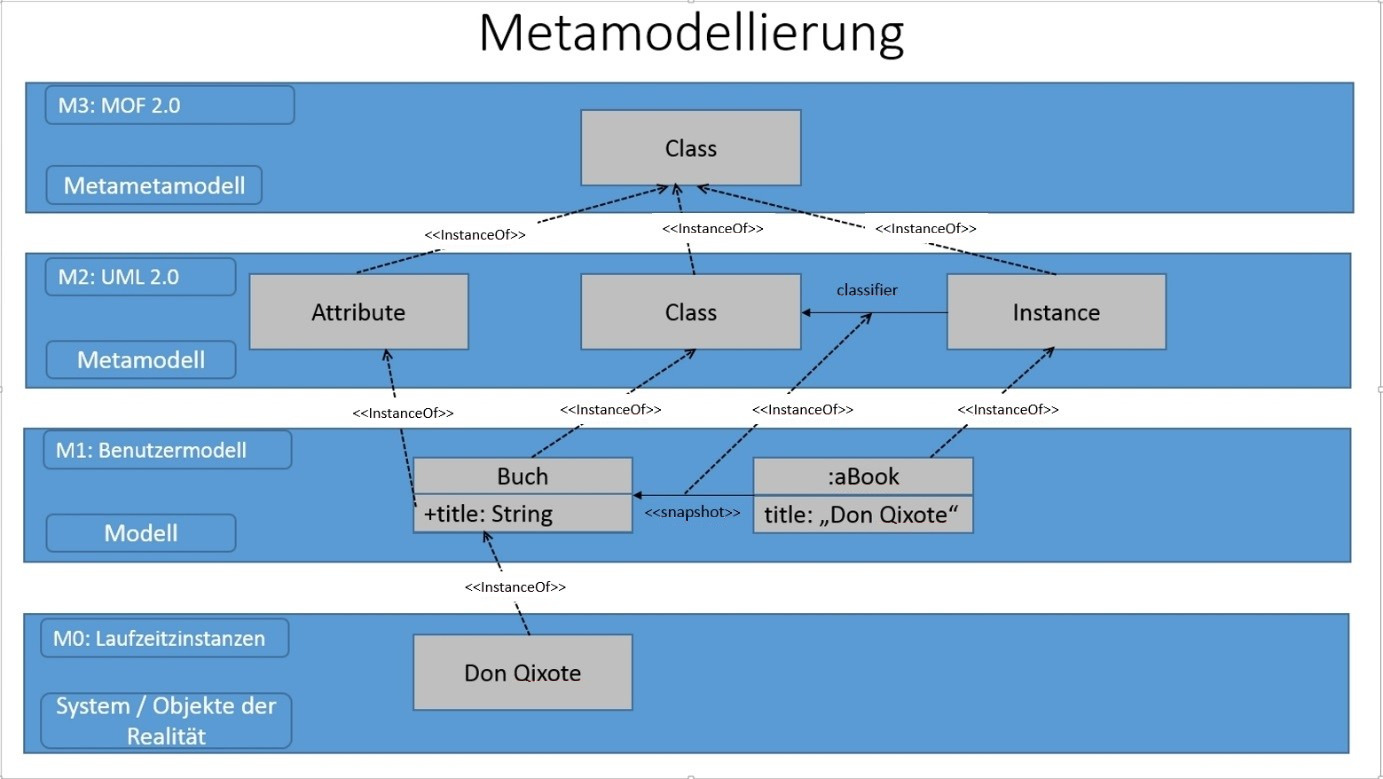
\includegraphics[scale=0.7]{Graphics/metamodell}
\captionof{figure}{Die Metamodellierung zeigt die hierarchische Beziehung zwischen den Sprachebenen}
\label{fig1}


Die obere Grafik zeigt die Metamodellierung von UML 2.0. Ebene M0 ist die grundlegende Ebene. Sie stellt konkrete, reale Objekte und einzelne Datensätze dar – z. B. ein Objekt oder eine Komponente. Ebene M1 umfasst alle Modelle, die die Daten der Ebene M0 beschreiben und strukturieren \cite{MT009}. Das sind UML-Diagramme wie das Aktivitätsdiagramm oder das Paketdiagramm (weiter unten erklärt). Um den Aufbau dieser Modelle zu definieren, legen Metamodelle der Ebene M2 die Spezifikationen und Semantik der Modellelemente fest.\\

Wollen Sie ein verständliches UML-Diagramm erstellen, müssen Sie das Metamodell UML mit seinen Regeln kennen. Die höchste Ebene, M3, ist ein Metamodell des Metamodells. Die erwähnte Meta Object Facility arbeitet auf einer abstrakten Ebene, die Metamodelle definiert. Diese Ebene definiert sich selbst, da sonst weitere, übergeordnete Meta-Ebenen entstünden.\\

\subsection{Kurzbeschreibung}
Bei der Unified Modeling Language (UML) handelt es sich nicht um eine bestimmte Methode, sondern vielmehr um einen Sammelbegriff für grafische Methoden der objektorientierten Entwicklung und Dokumentation von Software (Object Oriented Design – OOD). Dies umfasst Methoden und Notationen für Planung, Design, Entwurf und Implementierung von Software, die seit den 90er Jahren durch die Object Management Group (die auch BPMN pflegt) zu einem offiziellen Standard, der UML, zusammengeführt wurden.\cite{MT005} \\
Im Gegensatz zu anderen Methoden, die primär auf die Modellierung von Prozessen abzielen, kann die UML direkt zur Software-Entwicklung genutzt werden.\\
Die objektorientierte Sichtweise, auf der UML basiert, zieht ausgehend von der realen Welt Objekte heraus, die mit Attributen beschrieben werden. Die Objekte werden zu Klassen verdichtet, wenn Eigenschaften und Verhalten der Objekte identisch oder ähnlich sind. Klassen können daher als Baupläne für die zu erzeugenden Objekte (die Instanzen einer Klasse) interpretiert werden. Die Objekte, Klassen, Attribute und Methoden bilden die Basis für sämtliche Diagrammtypen der UML. Die verschiedenen Diagrammtypen können in\\

 statische Modelle (-> Strukturdiagramme)\\
• das Klassendiagramm,\\
• das Kompositionsstrukturdiagramm (auch: Montagediagramm),\\
• das Komponentendiagramm,\\
• das Verteilungsdiagramm,\\
• das Objektdiagramm,\\
• das Paketdiagramm und\\
• das Profildiagramm.\\
und\\
 dynamische Modelle (-> Verhaltensdiagramme)\\
• das Aktivitätsdiagramm,\\
• das Anwendungsfalldiagramm (auch: Use-Case o. Nutzfalldiagramm),\\
• das Interaktionsübersichtsdiagramm,\\
• das Kommunikationsdiagramm,\\
• das Sequenzdiagramm,\\
• das Zeitverlaufsdiagramm und\\
• das Zustandsdiagramm\\
unterteilt werden.\\
Statische Modelle (wie z.B. das Klassendiagramm) zeigen die Beziehungen zwischen den Klassen und den beteiligten Akteuren auf. Demgegenüber zeigen dynamische Modelle (wie z.B. das Sequenzdiagramm) den Prozessablauf auf. Aufgrund der Vielzahl an Diagrammtypen ergeben sich vielfältige Anwendungsmöglichkeiten, da jeder Typ eine spezifische Sicht auf den zu modellierenden Prozess sowie das System ermöglicht\cite{MT009}.\\
Im Folgenden werden einige ausgewählte UML-Diagrammtypen erläutert, wobei jeweils der Nutzen im Rahmen des Geschäftsprozessmanagements herausgearbeitet wird.\\
\\
\\
\\
Das Anwendungsfalldiagramm (use case diagram) dient im Rahmen der Softwareentwicklung dem Einstieg in die Anforderungsanalyse. Gleichzeitig kann es zur Darstellung der relevanten Geschäftsprozesse einschließlich der Beziehung zu den an den Prozessen beteiligten Personen genutzt werden. Ein Anwendungsfall entspricht hierbei entweder einem Geschäftsprozess oder einem Teilprozess. Durch das Anwendungsfalldiagramm kann dann dargestellt werden, welche Akteure an den betrachteten Prozessen beteiligt sind und welche Prozesse weitere Prozesse beinhalten. Die Akteure sind dabei im Sinne von Rollen eines Benutzers innerhalb des Systems zu verstehen, wobei diese nicht zwingend menschlich sein müssen. Dies ist beispielsweise der Fall, wenn ein anderes System eingebunden wird. Die Anwendungsfälle werden in diesem Diagrammtyp über Ellipsen abgebildet, während die Akteure als Strichmännchen dargestellt werden. Die Beziehungen zwischen dem Anwendungsfall und den beteiligten Akteur werden über ungerichtete Kanten visualisiert.\\



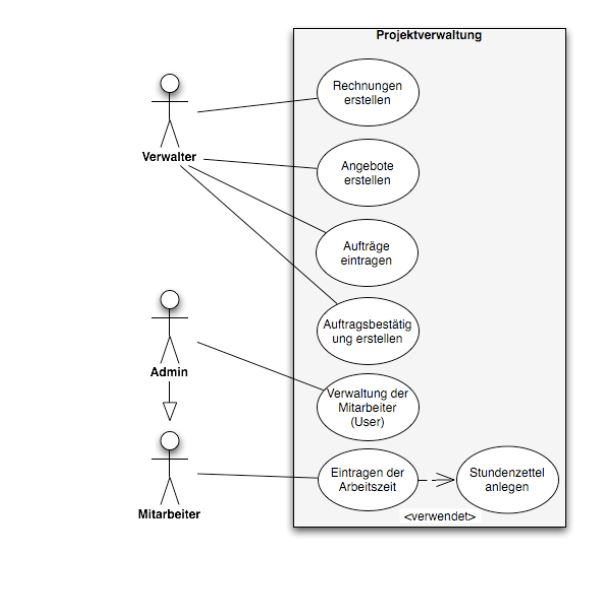
\includegraphics[scale=0.8]{Graphics/Anwendungsdiagram.jpg} 
\captionof{figure}{Beispiel eines Anwendungsfalldiagramms in UML}
Quelle : \cite{MT005}


Anwendungsfalldiagramme weisen jedoch den Nachteil auf, dass keine Reihenfolge bei der Bearbeitung der Anwendungsfälle abgebildet werden kann. Es wird somit nicht deutlich, welcher Anwendungsfall vor einem anderen durchgeführt werden muss. Allerdings kann diese Reihenfolge beispielsweise durch andere Methoden der UML, wie das Aktivitätsdiagramm, kompensiert werden. Zudem muss jeder Anwendungsfall anhand einer Beschreibung dokumentiert werden. Hierbei bestehen jedoch keine Vorgaben, weshalb sich Inkonsistenzen und Redundanzen ergeben können. Darüber hinaus kann nicht sichergestellt werden, dass Dritte die Dokumentation auch verstehen. Daher sollte auf Vorlagen, die nicht offiziell zum Standard der UML gehören, zurückgegriffen werden.\cite{MT005} \\


Das Klassendiagramm (Class Diagram) eignet sich zur Darstellung von Klassenstrukturen innerhalb eines IKS. Klassendiagramme können nicht direkt für die Geschäftsprozessmodellierung verwendet werden. Stattdessen handelt es sich eine statische Darstellung von Klassen, Objekten und deren Beziehungen untereinander. Klassendiagramme beschreiben jedoch nur, dass eine Interaktion besteht; wie diese ausgestaltet ist kann jedoch nicht dargestellt werden.\\


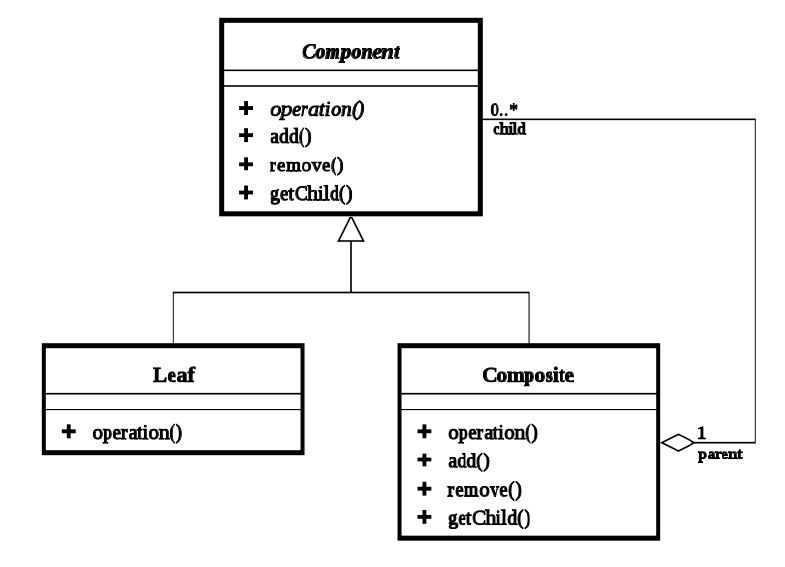
\includegraphics[scale=0.7]{Graphics/Klassendiagram.jpg} 
\captionof{figure}{Beispiel eines Klassendiagramms in UML}



Quelle : \cite{MT005}


Das Aktivitätsdiagramm oder auch Ablaufdiagramm (Activity Diagram) wird zur Darstellung von Abläufen verwendet. Im Mittelpunkt steht dabei die Visualisierung paralleler Abläufe\cite{MT005}. Aus diesem Grund eignet sich dieser Diagrammtyp in einem besonders hohen Maße zur Abbildung von Geschäftsprozessen, da diese zumeist Parallelitäten vorweisen. Aktivitätsdiagramme sind darüber hinaus zur Modellierung von Workflows und zur Verfeinerung von Anwendungsfällen geeignet. Des Weiteren sind Aktivitätsdiagramme in der Lage unterschiedliche Detaillierungsgrade wiederzugeben. So ist es unter anderem möglich ein anwendungsfallübergreifendes Diagramm zu erzeugen und anschließend die darin enthaltenen Anwendungen einzeln zu modellieren.\\

   

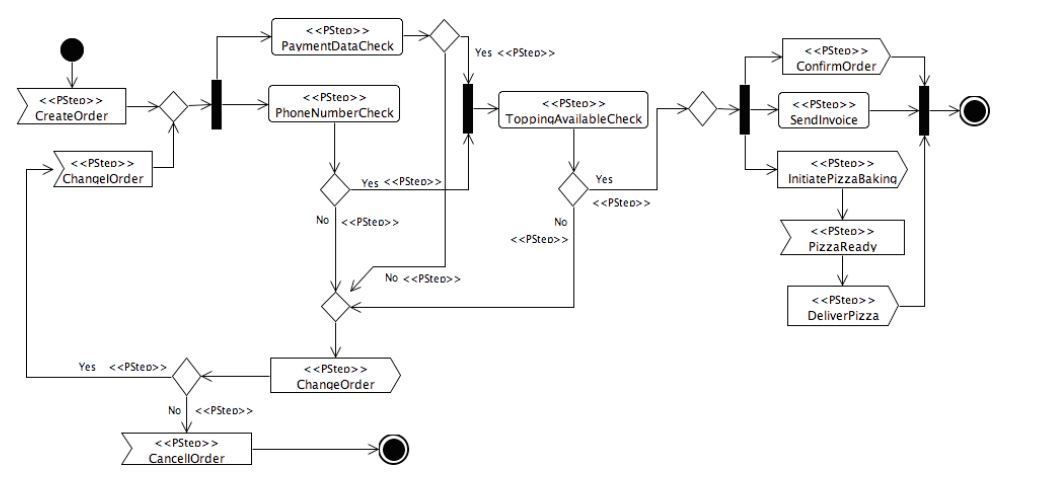
\includegraphics[scale= 0.65]{Graphics/activitydiagram.jpg} 
\captionof{figure}{Beispiel eines Aktivitätsdiagramm in UML}



Quelle : \cite{MT005}


\subsection{UML-Diagramme: Eine Übersicht}
Die folgende Übersicht zeigt übergeordnete Kategorien und Anwendungsmöglichkeiten der einzelnen Diagrammtypen in Kurzform. Wenn Sie ein modellorientiertes Software-System, einen Anwendungsfall in der Wirtschaft o. Ä. visuell darstellen wollen, sollten Sie laut Empfehlung der UML-Task-Force vorher einen der UML-Diagrammtypen wählen. Erst dann lohnt es sich, eines der vielen UML-Tools zu wählen, da diese häufig eine gewisse Methode vorschreiben. Dann erstellen Sie das UML-Diagramm.\cite{MT011} \\

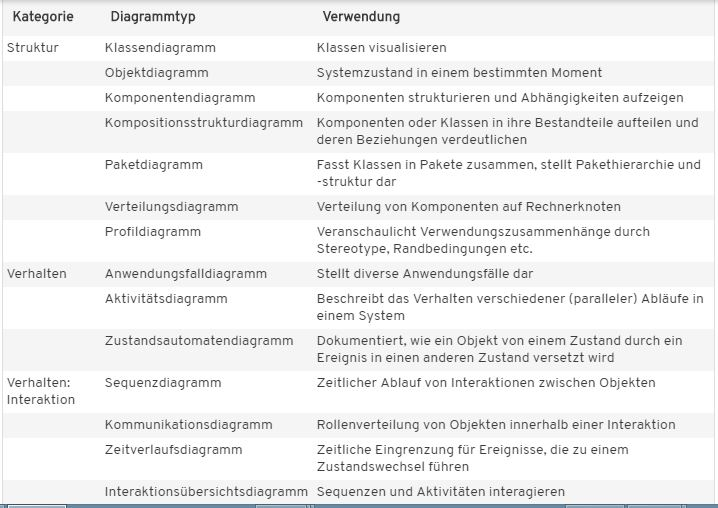
\includegraphics[scale=1]{Graphics/UMLdiagramme.jpg} 
\captionof{figure}{UML-Diagramme}


 

\subsection{Vor- und Nachteile im Überblick}
UML ist heute eine der dominierenden Sprachen für die Modellierung von betrieblichen Anwendungs- bzw. Softwaresystemen. Der erste Kontakt zu UML besteht häufig darin, dass UML-Diagramme im Rahmen von Softwareprojekten zu erstellen, zu verstehen oder zu beurteilen sind\cite{MT005}. UML-Diagramme gelten als Standard bei objektorientierter Modellierung.\\

   

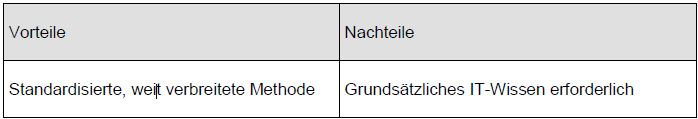
\includegraphics[scale=0.9]{Graphics/vornach.jpg}
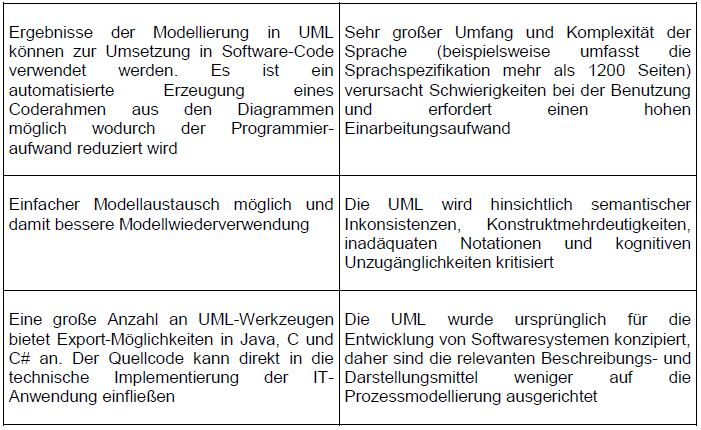
\includegraphics[scale=0.9]{Graphics/vornach2.jpg} 
\captionof{figure}{UML: Vor- und Nachteile }


Quelle : \cite{MT005} 

 


\section{MSC}
\label{sc:MSC}
MSC ist von der International Telecommunication Union (ITU) normierte Sprache.  Sie hat eine graphiseche Notation, um den Benutzer zu darstellen, und eine textuelle Notation für die Bearbeitung durch Software-Werkzeuge, genauso wie bei SDL.
MSC bietet die Möglichkeit, das Kommunikationsverhalten zwischen Systemkomponenten und deren Umgebung zu beschreiben. Diese Kommunikations ist auf den Austaush von Nachrichten basiert.
Mit Msc-Specifikationen können unterschiedliche Sichten auf das Systemverhalten erzeugt werden. 
Dazu gibt MSC einen globalen Einblick auf das System aus, wie zum Beispiel die Interaktionen von alle Instanzen.\\
MSC und UML haben fast das gleiche Prinzip und man kann sogar als Variante von MSC den Sequence Diagrams in UML integrieren.
Trotz der vielen Gemeinsamkeiten von dieser drei Modellierungssprachen (UML, SDL und MSC), haben sie viele große Unterschied in dem tatsächlichen Entwurf. Beispielsweise kann man mit MSC nur Beispielabläufe und kein vollständig System beschreiben.\\
Die MSC-Diagramme sind in den frühen Phasen hilfreich, wobei können sie erste Ideen und Einblick zum System anzeigen.
Damit kann man einfach in der Entwurfsphase wichtige erwünschte oder unerwünschte Beispielabläufe bemerken oder in späteren Phasen den Testzweck schauen, der von die MSC-Diagramme genau definiert wurde.\\

Die wichtigsten Konstrukte und Elemente der MSC werden in diesem Abschnitt anhand ein Beispiel dargestellt. Wir glauben, dass ein Beispiel das beste Weise ist, um Das MSC Konzept zu erklären und zu definieren. 
Das folgende Beispiel beschreibt einen Prozess, der aus vier verschiedenen Einzelteilen (A, B, C und D) zwei Produkte von Typ AC oder BDC produziert. 


\subsection{Basic-MSC}
Das erste wichtige Teil von MSC ist ein Basic-MSC. Ein Basic-MSC umfasst alle notwendige Srachkonstrukte zur Spezifizierung des Nachrichtenfluss.
Die Sprachkonstrukte von einem einfachen MSC (Basic MSC9 sind: Instanz, Message, Environment, Action, Timer-Start, Timeout, Timer-Stop, Create, Stop und Condition. \\
Das wichtigste Teil vom Basic-MSC sind den Nachrichtenaustausch. Diese Nachrichten können verschiedene Parameter tragen, die den Typ einer Nachricht unterscheiden. Auf dieser Weise sind zwei Nachrichten gleich, wenn sie den gleichen Inhalt besitzen.
Ein Basic-MSC definiert eine partielle Ordnung auf Ereignissen, die an einem Ort (heißt Instanz) stattfinden.
Diese Ereignissen können in verschiedenen Fromen erscheint werden, zum Beispiel: Kommunikationsereignisse ( wie das Senden und Empfangen einer Nachricht), Timer-Ereignisse, lokale Aktionen oder das Erzeugen einer Instanz.\\
Um ein Basic-MSC besser zu erklären, ist ein Beispiel davon in der nächsten Abbildung gezeigt.
Ein Basic-MSC mit dem Namen ProduktionAC ist in
Abbildung 1.6 gezeigt.
\begin{center}
\begin{figure}[h]
   

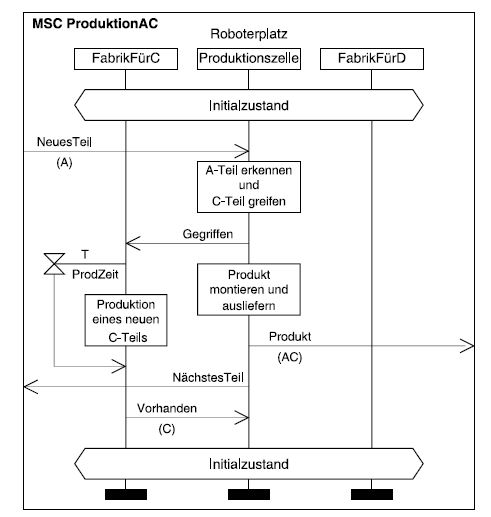
\includegraphics[scale=1]{Graphics/MSC1.jpg}

\captionof{figure}{Ein Basic-MSC}


Quelle : \cite{MT009}
Part 1: Message Sequence Chart (MSC) 

 
\label{fig7}


\end{figure}

\end{center}
\newpage
Der Name von diesem Basic-MSC ist ProduktionAC und er muss oben in der Ecke geschrieben werden. Das Basic-MSC in diesem Beispiel beschreibt die Produktion eines Produkts, das aus einem A-Teil und einem C-Teil zusammengesetzt ist.
Die wichtige Elemente in dieser Abbildung sind: Der Produktionszelle, FabrikfürC und Fabrik von D. Das MSC beschreibt ein detaillierte Szenario vom Informationsaustausch zwischen diese drei Element. 

\\
Am Anfang ist der Produktionsprozess in seinem Initialzustand, Der ein benötige Bedingung für die nächste Aktionen ist. 
 Das System ist initialisiert und Teile
der Typen C und D sind gefertigt, eingelagert und der
Produktionszelle zur Verfügung gestellt worden.
 Die Systemumgebung schickt das A-Teil an die Produktionszelle.
 Danach erkennt die Produktionszelle das empfangende Teil, greift das für die Produktion notwendige C-Teil und meldet das Entfernen des
 C-Teils vom Greifplatz an die FabrikfürC, die für das C-Teile zuständig ist. 
 Beim letzten Schritt wird ein Produkt von Typ AC produziert, ausgegeben und zu die Systemumgebung geschickt.
Danach meldet die Produktionszelle die Bereitschaft
für die Bearbeitung des nächsten A- oder B-Teils
an die Systemumgebung.
In der Gleichzeitig wird ein neues C-Teil wieder produziert und es ist jetzt verfügbar für die nächste Produktion.

\subsubsection{Instanz und Message}
Instanzen und Nachrichten (Message) sind die wichtigste Sprachkunstrukte von Basic-MSC.

Instanzen sind Komponenten, die mit der Systemumgebung oder untereinander
asynchron Nachrichten austauschen können.\\
Die Instanzen sind als vertikale Linien dargestell. Am Enfang dieser Linier findet man der Instanzkopf, wo der Instanzname spezifiziert wird. Zusätzlich kann man noch direkt über den Instanzkopf ein Typ zu dieser Instanz angeben (z.B. Instanz Produktionszelle vom Typ Roboterplatz in Abbildung).
Die Linie der Instanzen endet sich mit einem Instanz-Ende-Symbol. Ein Instanz-End bedeutet, dass es in dem MSC keine weiteren Ereignisse für diese Instanz gibt, aber das bedeutet nicht unbedingt, dass die Instanz gestoppt ist.\\


Die Nachrichten werden durch Pfeile dargestellt. Die Pfeile
können horizontal oder geneigt sein, um den Zeitverlauf
anzuzeigen. 
Jede Nachricht definiert definiert genau zwei Eereignisse: Das Senden der Nachricht ist durch den Pfeileanfang beschrieben und die Pfeilspitze bezeichnet
die Verarbeitung einer Nachricht.
Jede Nachricht hat einen Name und optionale Nachricht-Parametern, die in Klammern angegeben werden müssen (Zum Beispiel in Abbildung hat die erste Nachricht den Name NeuesTeil mit dem Parameter A).
 Bei Jeder Instanzlinie gibt es eine Totalordnung der der spezifizierten
 Message-Sende- und Message-Verarbeitungsereignisse. Dazu gibt es zwischen die verschieden Instanzachse partiell Ordnung, wobei sollte eine Nachricht zuerst gesendet werden, bevor sie empfängt wird. 

\subsubsection{Environment}
Die Systemumgebung ist durch die Diagrammfläsche eines MSC definiert. Diese Diagrammfläsche wird durch einen rechteckigen Rahmen begrenzt.
die Systemumgebung und heißt Environment. Nachrichten,
die aus der Systemumgebung kommen oder an die Systemumgebung
gesendet werden, beginnen und enden auf
dem Environment (z.B. die Messages NeuesTeil und
Produkt in Abbildung). Die Sende- und Verarbeitungsereignisse aus und an die Systemumgebung definieren in der Regel keine Ordnung.

\subsubsection{Action}

Aktionen von Instanzen können ind Form von Actions spezifiziert werden.
Eine Action wird durch ein Rechtecksymbol dargestellt, der Name der Aktion enthalten kann (z.B. Action ,Produkt
montieren und ausliefern‘ in Abbildung).
\\
\subsubsection{Timer}
Die Sprachkonstrukte Timer-Start, Timeout und Timer-Stop können zusätzlich die Timern beschreiben, damit wird es deutlicher den Anfang und das Ende der Aktionen definiert.
Der Anfang der Pfeile(mit Sanduhr-Symbol) definiert das Time-Start und das Ende der Pfeile definiert das Timeout. Zusätzlich muss man den Name von Timer und optional die Timer-Parametern definieren.

Ein Timer-Start und seine Timeout werden
in Bild Abbildung verwendet, um die Produktionszeit für ein Teil des
Typs C zu modellieren.In diesem Fall hat der Timer hat den Namen T und
den Parameter Prodzeit.\\
\subsubsection{Condition}
Die Beschreibung vom Zustand definiert durch Condition ( Bedingung)
Graphisch werden Conditions durch Sechsecke dargestellt,
die die Instanzen, auf die sich die Condition bezieht,
überdecken. Conditions werden zur Beschreibung von
wichtigen Systemzuständen benutzt. In Abbildung befinden sich
zwei Conditions, die Initialzustand heißt und den globalen Systemzustand beschreiben.\\


\subsection{Strukturelle Sprachkonstrukte}
Strukturelle MSC-Sprachkonstrukte bezeichnen Sprachelemente,
die über die Beschreibung des reinen Messageflusses
hinausgehen. Mit ihnen lassen sich MSCs und
MSC-Teile zu komplexeren Abläufen kombinieren (Inline-
Expressions und High-Level-MSC), MSC-Diagramme in
anderen MSC-Diagrammen wiederverwenden (References),
MSC-Instanzen verfeinern (Decomposition) und allgemeine
Ereignisstrukturen für Instanzen definieren (Coregion und
General Ordering).\cite{MT009}\\

\begin{center}
\begin{figure}[h]
   

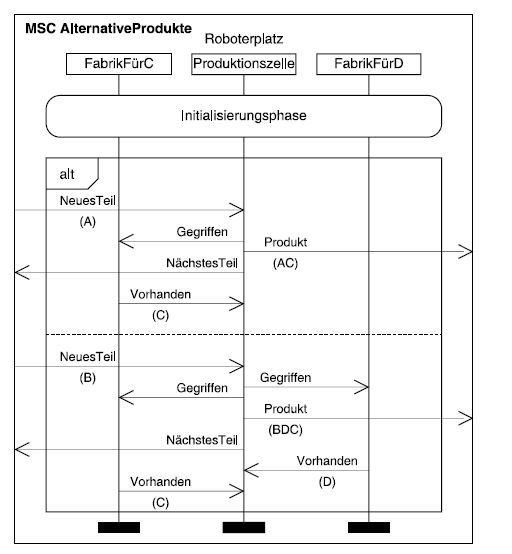
\includegraphics[scale=1]{Graphics/MSCmit.jpg}

\captionof{figure}{MSC mit strukturellen Sprachkonstrukten }


Quelle : \cite{MT009}
Part 1: Message Sequence Chart (MSC) 

 
\label{fig8}


\end{figure}

\end{center}
\newpage
\subsubsection{Inline-Expressions}
Inline-Expression werden als Operatoren in MSCs definiert. Damit können Teilabläufe,
die innerhalb eines MSC-Diagramms spezifiziert worden sind, zu komplexeren Abläufen kombiniert werden. Sie erlauben es, die Wiederholung von Teilabläufen (loop-Operator),
alternative Teilabläufe (alt-Operator), die parallele Komposition von Teilabläufen (parOperator), optionale Teilabläufe (opt-Operator) und Ausnahmen in Form von Teilabläufen (exc-Operator) zu spezifizieren. Graphisch werden Inline-Expressions als Rechtecke mit in der linken oberen Ecke spezifizierten Namen dargestellt. Teilabläufe werden durch gestrichelten Linien in Sections separiert.
\subsubsection{References}
References ermöglichen es, MSCs in anderen MSCs wieder
zu verwenden. 
Ein Reference unterscheidet und referenziert die andere MSC mit dessen Namen. 
Die References sind mit abgerundeten Rechteck dargestellt (z.b Ein Reference ist mit dem Name Initialisierungsphase in Abbildung dargestellt).\\


\subsection{High-Level-MSC}
High-Level-MSC ist auch als (HMSC) bekannt. Es ermöglicht eine kombinierte Darstellung von mehren MSCs auf abstrakter Ebene. Diese Kombination ist durch gerichteten Graphen beschriebt. Die Knoten eines HMSC-Diagramms sind ein Anfangsknoten, Endknoten, Konnektoren, References und Conditions.
\\ HMSC gibt ein globale Einblick von der gesamten Kombination von MSC-Diagrammen, damit kann man parallele, sequentielle alternative
Kombination von MSCs in einer Einzige Abbildung und in einer sehr intuitiven Form beschreiben.\\•



\begin{center}
\begin{figure}[h]
   

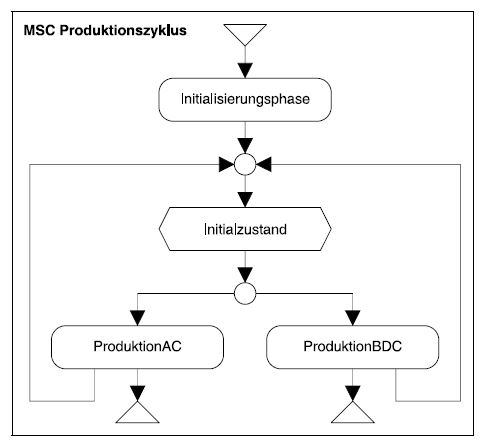
\includegraphics[scale=1]{Graphics/HMSC.jpg}

\captionof{figure}{Ein High-Level-MSC }


Quelle : \cite{MT009}
Part 1: Message Sequence Chart (MSC) 

 
\label{fig9}


\end{figure}

\end{center}
\newpage
In der Abbildung beschreibt das HMSC-Beispiel, die verschiedene Szenarien, die im Produktionsprozess-Beispiel passieren können. 
Die verschieden Szenarien in dieser Abbildung sind:Am Anfang gibt es direkt die Initialisierungsphase,danach
befindet sich der Produktionsprozess in seinem
Initialzustand. Im Initialzustand können entweder Produkte
vom Typ AC oder vom Typ BCD hergestellt werden. Nach
der Herstellung eines Produkts befindet sich der Produktionsprozess
wieder im Initialzustand und ein neues Produkt
kann entweder gefertigt werden oder der Produktionsprozess endet.

\subsection{Weitere Sprachkonstrukte}
Wir haben in diesem Abschnitt dieses Kapitel nur an die sichtigsten Elemente der MSC-Sprache konzentriert. Damit haben wir ein globale aus ausreichende Einblick, um diese Modellierungssprache zu bewerten. Aber dazu gibt es noch weitergehende Konzepte, die MSC zu einer vollständigen Spezifikationssprache machen







